% %%%%%%%%%%%%%%%%%%%%%%%%%%%%% TCC %%%%%%%%%%%%%%%%%%%%%%%%%%%%%%%%
% %
% % Instituto Federal do Maranhão - Campus Caxias
% %
% % Autor: Leonardo Almeida de Araújo
% % 
% %%%%%%%%%%%%%%%%%%%%%%%%%%%%%%%%%%%%%%%%%%%%%%%%%%%%%%%%%%%%%%%%%%%

\documentclass{configuracoes}

% Alterar o arquivo a_dados_tcc.tex
%%%%%%%%%%%%%%%%%%%%%%%%%%%%%%%%%%%%%%%%%%%%%%%%%%%%%%%%%%%%%%%%%%%%%%%%%%%
% Dados do Arquivo
%%%%%%%%%%%%%%%%%%%%%%%%%%%%%%%%%%%%%%%%%%%%%%%%%%%%%%%%%%%%%%%%%%%%%%%%%%%

% Cidade
\newcommand{\cidade}{Caxias}
% Estado 
\newcommand{\estado}{Maranhão}
% Sigla do estado
\newcommand{\siglaestado}{MA}

%%%%%%%%%%%%%%%%%%%%%%%%%%%%%%%%
% Informações sobre departamento
%%%%%%%%%%%%%%%%%%%%%%%%%%%%%%%%

\newcommand{\instituto}{Instituto Federal do Maranhão}

% digitar o nome do departamento (dep)
\newcommand{\dep}{Departamento de Ensino Superior e Tecnológico}

% sigla do departamento
\newcommand{\sigladep}{IFMA}

%%%%%%%%%%%%%%%%%%%%%%%%%%%%%
% Informações sobre o curso 
%%%%%%%%%%%%%%%%%%%%%%%%%%%%%
% Titulacao do curso
\newcommand{\titulacao}{Bacharel}
% Nome do curso
\newcommand{\nomedocurso}{Ciência da Computação}

%%%%%%%%%%%%%%%%
% Sobre o autor
%%%%%%%%%%%%%%%%
% Nome do autor
\author{Leonardo Almeida de Araújo}
% Titulo do trabalho
\title{Utilização de Redes Neurais para a detecção de ataques em ambientes IoT domésticos baseado no comportamento do tráfego de rede}
% Subtitulo do trabalho
\newcommand{\subtitulo}{Subtitulo}
% \newcommand{\subtitulo}{} % quando não existir

%%%%%%%%%%%%%%
% Orientador 
%%%%%%%%%%%%%%
% Nome do Orientador
\renewcommand{\orientador}{Profº.: Me.: Josenilson Dias
Araújo}

% Orientador - comentar para alterar
\newcommand{\genorientador}{Orientador} % masculino
% \newcommand{\genorientador}{Orientadora} % feminino

% Coorientador - comentar para alterar
\renewcommand{\coorientador}{} % quando não existir
\renewcommand{\coorientador}{Coorientador} % masculino
% \renewcommand{\coorientador}{Coorientadora} % feminino

% Nome do coorientador
\newcommand{\nomecoorientador}{Prof.: Dr.: Ramon Santos Nepomuceno}

%%%%%%%%%%%%%%%%%%%%%%%
% banca de examinadora
%%%%%%%%%%%%%%%%%%%%%%%
% Membros da Banca
\newcommand{\profb}{Membro da Banca 1}
\newcommand{\instprofb}{Instituto do Membro da Banca 1}

\newcommand{\profc}{Membro da Banca 2}
\newcommand{\instprofc}{Instituto do Membro da Banca 2}


\begin{document}
 \pretextual
 \begin{figure}[h]
\centering

\includegraphics[scale=0.3]{imagens/logo.png}
\end{figure}

\begin{center}
\MakeUppercase{\dep} \hspace*{2mm}- \sigladep \\
  \MakeUppercase{\nomedocurso}
\end{center}

  \vspace*{2in}
  \begin{center}
    \LARGE\textbf{ \thetitle}\\
    %\Large\textbf{ \subtitulo}\\
  \end{center}

  \vspace*{1in}

  \begin{center}
    {\MakeUppercase \theauthor}
  \end{center}

\vspace{1.5in}

\begin{samepage}
    \begin{center}
    \cidade \hspace*{2mm}- \siglaestado \\ \the\year
    \end{center}
\end{samepage}


\begin{center}
  {\MakeUppercase \theauthor}
\end{center}

\vspace{2in}

\begin{center}
  {\huge \thetitle}\\
  %\subtitulo
\end{center}

\vspace{1in}

\begin{flushright}
    \begin{minipage}{0.5\textwidth}
    Monografia apresentada ao curso \nomedocurso \hspace{1mm}do \dep, do \instituto, como requisito para a obtenção do grau de \titulacao \ em \nomedocurso
    \end{minipage}
    
    \vspace*{0.2in}
    
    \begin{minipage}{0.5\textwidth}
       \begin{minipage}[t]{0.35\textwidth}
        \genorientador
       \end{minipage}
       \begin{minipage}[t]{0.6\textwidth}
        \orientador
       \end{minipage}\\
       
       \begin{minipage}[t]{0.35\textwidth}
        \coorientador
       \end{minipage}
       \begin{minipage}[t]{0.6\textwidth}
        \nomecoorientador
       \end{minipage}
    \end{minipage}

\end{flushright}
\vspace*{1in}

\begin{center}
    \Month \\ \the\year
\end{center} % Não necessita de alterações
 
 % % Isto é um exemplo de Ficha Catalográfica, ou ``Dados internacionais de
% catalogação-na-publicação''. Você pode utilizar este modelo como referência. 
% Porém, a biblioteca da universidade lhe fornecerá um PDF com a ficha catalográfica definitiva após a defesa do trabalho. Quando estiver com o documento, salve-o como PDF na pasta pdf do seu projeto e substitua todo o conteúdo de implementação deste arquivo pelo comando abaixo:

% \begin{fichacatalografica}
%     \includepdf{pdf/ficha_catalografica.pdf}
% \end{fichacatalografica}

% Comente ou retire todas as linhas abaixo após inserir o documento da ficha catalográfica

\begin{fichacatalografica}
	\sffamily
	\vspace*{2in}					% Posição vertical
    
	\begin{center}					% Minipage Centralizado
    	\fbox{
    	    \begin{minipage}[c][8cm]{13.5cm}		% Largura
            	\small
            	\imprimirautor
            	%Sobrenome, Nome do autor
            	
            	\hspace{0.5cm} \imprimirtitulo  / \imprimirautor. --
            	\cidade, \estado - 
            	
            	\hspace{0.5cm} \thelastpage p. : il. (algumas color.) ; 30 cm.\\
            	
            	\hspace{0.5cm} \genorientador~\orientador\\
            	
            	\hspace{0.5cm}
            	\parbox[t]{\textwidth}{Trabalho de Conclusão de Curso~--~IFMA - Caxias/MA,
            	\Month de \the\year.}\\ 
            	
            	\hspace{0.5cm}
            		1. Palavra-chave1.
            		2. Palavra-chave2.
            		2. Palavra-chave3.
            		I. Orientador.
            		II. Universidade xxx.
            		III. Faculdade de xxx.
            		IV. Título 			
        	\end{minipage}
    	}
	\end{center}

\end{fichacatalografica}
 
 
 % Ficha de aprovação - necessita de alterações casuais, para mais informações acessar o arquivo 01_ficha_aprovação.tex
 % \newpage
 % 
% Isto é um exemplo de Folha de aprovação, elemento obrigatório da NBR 14724/2011 (seção 4.2.1.3). Você pode utilizar este modelo até a aprovação do trabalho. Após isso, quando estiver com o documento com todas as assinaturas, salve-o como PDF na pasta pdf do seu projeto e substitua todo o conteúdo de implementação deste arquivo pelo comando abaixo:

% \begin{folhadeaprovacao}
% \includepdf{pdf/folhadeaprovacao_final.pdf}
% \end{folhadeaprovacao}

% Comente ou retire todas as linhas abaixo após inserir o documento da ficha de aprovação

\begin{folhadeaprovacao}

\begin{center}
\sigladep \hspace{2mm}- \dep \\
\instituto
\end{center}

\vspace{0.2in}

Trabalho de Conclusão de Curso de \nomedocurso \hspace*{0.1mm} intitulado \textit{\textbf{\em \thetitle}} de autoria de \theauthor, 
aprovada pela banca examinadora constituída pelos seguintes professores: 

\vspace{1in}

\begin{center}
 \begin{minipage}{0.6\textwidth}
  \hrule \vspace{0.05in}
  \orientador \\
  \genorientador\\
 \end{minipage}
  
  \vspace{1in}
 \begin{minipage}{0.6\textwidth}
  \hrule \vspace{0.05in}
  \profb\\
  \instprofb\\
 \end{minipage}
 
 \vspace{1in}
 \begin{minipage}{0.6\textwidth}
  \hrule \vspace{0.05in}
  \profc\\
  \instprofc\\
 \end{minipage}
\end{center}

\vfill

\begin{center}
\cidade, \today
\end{center}

\vspace{0.05in}

\newpage
\end{folhadeaprovacao}
 
 
 %Dedicatoria
 % \section*{Dedicatória}
 % \begin{dedicatoria}
 %   
    ***A dedicatória é opcional***
 % necessita de alterações
 % \end{dedicatoria}
 
 %Agradecimentos
 % \begin{agradecimentos}
 %   
    ***O agradecimento é opcional***
 % necessita de alterações
 % \end{agradecimentos}
 
 %Epigrafe - comentar linha de baixo caso nao existe necessidade de epigrafe
 % \begin{epigrafe}
 %   \vspace*{\fill}
 %	\begin{flushright}
 % 	    
 *** A epígrafe é opcional ***
 % necessita de alterações
 % 	\end{flushright}
 % \end{epigrafe}
 
 %\setlength{\absparsep}{18pt} % ajusta o espaçamento dos parágrafos do resumo
 %\begin{resumo} % inserir resumo
 %   

\textbf{ Palavras-chave:} 
\key{Machine Learning},  
\key{Segurança de dados}, 
\key{Redes domésticas}. % necessita de alterações
 %\end{resumo}
 
% \begin{resumo}[abstract] % inserir abstract
%   \begin{otherlanguage*}{english}
%     
\textbf{Key-words:} 
\key{Machine Learning},  
\key{Networks Security}, 
\key{Domestic Networks}. % necessita de alterações, devem estar em ingles
%   \end{otherlanguage*}
% \end{resumo}
 
 %Lista de figuras%
 %\renewcommand{\listfigurename}{Lista de Figuras}
 %\listoffigures
 
 \begin{siglas}
  \item[IFMA] Instituto Federal do Maranhão
  \item[IDS] Sistema de Detecção de Intrusão
  \item[IoT] Internet das Coisas
  \item [RNA] Rede Neural Artificial
  \item [IP] Protocolo de Internet
  \item [TCP] Protocolo de Controle de Transmissão
\end{siglas} % comentar caso nao seja usado

 % Sumario
  \tableofcontents*
  \cleardoublepage

\textual
 % Introdução
 \chapter{INTRODUÇÃO}
Dado o crescimento exponencial do uso da internet, em virtude da convergência de áreas para dentro da computação, aumenta-se a complexidade e a necessidade de se manter cuidadoso diante de problemas de segurança. \cite{mendes2020redes}

Antes, somente computadores e celulares eram conectados a internet, mas com a chegada dos dispositivos IoT (Internet of Things), permitiu-se que qualquer objeto seja conectado à rede, o que também abriu brechas para ainda mais problemas de segurança \cite{alrawi}.

 A IoT é uma rede de objetos físicos, que inclui desde utensílios domésticos como lâmpadas, veículos, sensores, câmeras de vigilanciana e outros objetos conectados com a Internet. No ano atual, existem cerca de 12.2 bilhões de dispositivos IoT ativos e espera-se que, até 2025, haverá aproximadamente 27 bilhões. \cite{Gomes_2022}; \cite{IoTResearch}.

Devido a este crescimento, necessita-se também de técnicas mais eficazes para garantir a integridade e segurança dos dados pessoais, visto que dispositivos IoT domésticos acabam sendo um alvo fácil devido sua baixa segurança \cite{Otoum}. Uma das técnicas de combater estes ataques é com o uso de IDSs.

Sistemas de Detecção de Intrusão (IDS), fazem a detecção de possíveis ameaças a partir da classificação de padrões ou comportamento do tráfego de rede \cite{Shurman}. Kitsune é um algorítimo baseado em Redes Neurais Artificiais não supervisionadas, open-source, capaz de aprender padrões e comportamentos complexos para diferenciar um trafego normal ou um ataque. \cite{kitsune}

A ideia de usar o monitoramento de pacotes de dados foi empregado pela primeira vez por James Anderson em 1980. A partir deste momento, pesquisadores desenvolveram vários métodos para melhorar o desempenho e precisão das analises. Uma opção é unir a capacidade de uma rede neural em processar padrões ao monitoramento de dados.

Pretende-se usar como base o algorítimo Kitsune \cite{kitsune}, e realizar uma pesquisa de aplicação e viabilidade do uso de Redes Neurais Artificiais para detectar intrusões em redes domésticas. % necessita de alterações 
 
 % Conceitos Gerais
 \chapter{PROBLEMA}
Diante do exposto, pretendemos realizar uma análise a respeito do uso de Redes Neurais Artificiais abordando o aprendizado não supervisionado para a detecção de intrusões em ambientes IoT domésticos, também responder a seguinte pergunta: Em relação ao desempenho e usabilidade, o uso de Redes Neurais Artificiais para proteção de redes domésticas é uma escolha viável?

\chapter{HIPÓTESES}
Com um software inteligente baseado em Redes Neurais, é possível reconhecer os padrões e comportamentos de uma rede doméstica, e diferenciar um trafego normal de um ataque.

\chapter{OBJETIVO GERAL}
Avaliar a eficiência da implementação de um Sistema de Detecção de Intrusão baseado em Redes Neurais Artificial não supervisionadas, em hardwares domésticos.

\section{OBJETIVOS ESPECÍFICOS}
\begin{itemize}
    \item Realizar a implementação do Sistema de Detecção de Intrusão para redes domésticas baseado no IDS Kitsune;
    \item Verificar o desempenho do IDS em hardwares comuns em residencias;
    \item Analisar a eficiência do IDS com ataques simulados em ambientes IoT Domésticos;
    \item Realizar uma investigação sobre a taxa de erro do algorítimo em ambientes IoT domésticos;
    \item Apresentar os resultados do Sistema de Detecção de Intrusão, para assim, validar a eficiência e precisão do algoritmo em ambientes domésticos; 
 \end{itemize}

\chapter{JUSTIFICATIVA}
Ao observarmos a complexividade da prevenção e detecção de ataques, visualizamos o problema da rápida e constante mudança da maneira que esses ataques acontecem. Por isso é essencial que os métodos de segurança sejam constantemente atualizados. Uma ferramenta útil são os Sistemas de Detecção de Intrusão (IDS), que são softwares que monitoram o tráfego, e tomam ações caso exista um comportamento incomum na rede.

Com a flexibilidade dos IDSs, é possível trabalhar em conjunto com outros sistemas, como Firewalls ou hardwares, ou integra-los a Redes Neurais Artificiais (RNA), possibilitado que eles tenham uma tomada de decisão e aprendizado.
Redes Neurais Artificiais não supervisionadas, são um ponto chave em IDSs, pois não se faz necessário o tempo e esforço para atualizar manualmente o Sistema de Detecção de Intrusão, já que o mesmo aprende de forma incremental a partir dos dados e padrões. 

Para que um IDS seja implementado em um ambiente domestico, é importante que ele exija pouco uso de processamento, pois na maioria dos casos, os hardwares domésticos são menos robustos e possuem um sistema simples. O algorítimo Kitsume, usa uma complexividade baixa em sua execução, trazendo um menor uso de processamento \cite{kitsune}.

Kitsune é um IDS baseado em Redes Neurais, que utilizaremos como base de pesquisa, pois além de ser um Software de código aberto, possui uma robusta abordagem de aprendizado não supervisionado, usando de Autoencoders para diminuir a complexidade dos processos.

Com esta pesquisa, espera-se contribuir com um relatório sobre a eficácia do método de aprendizado de máquina não supervisionado para soluções de segurança de redes domesticas, e apresentar um estudo aprofundado sobre o impacto de ataques de intrusão.

\chapter{REFERENCIAL TEÓRICO}
\section{Internet das Coisas (IoT)}
O termo Internet das Coisas se refere a conexão de vários objetos por meio da internet. Dispositivos IoT são capazes de interagir de maneira autônoma, possuindo uma capacidade “inteligente” de receber e processar informações pela rede. Em ambientes domésticos, estes dispositivos são responsáveis por automatizar tarefas do dia a dia \cite{gokhale2018introduction}.
 
\subsection{Segurança em IoT}
Com a vasta possibilidade de conexão em todo ambiente, aumentam também as vulnerabilidades a ataques. Dispositivos IoT muitas vezes não são projetados para terem um sistema robusto de segurança, pois o envio de informações precisa ser rápido, assim deixando as questões de segurança em segundo plano ou inexistentes. Nessas condições, estes dispositivos acabam sendo uma porta de entrada para ataques \cite{Anthi}. 

\hfill
\newcolumntype{L}{>{\RaggedRight\arraybackslash}X}
\begin{table}[!hbt]
\renewcommand\thetable{1}
\setlength\tabcolsep{3pt} 
\caption{Ataques comuns em redes IoT}
\centering
 \begin{tabularx}{\textwidth}{@{}*{4}{L} @{}} 
 \toprule
 Ataque & Alvo & Consequência & Técnica \\ [0.5ex]
 \midrule
 Negação de Serviço &
 Dispositivos IoT conectados a rede &
 Torna os dispositivos inacessíveis &
 Envia várias requests que nunca são completadas \\ 
 \addlinespace
 Wormholes &
 Localização dos pacotes de rede &
 Cria problemas de privacidades e nas rotas dos pacotes &
 Reencaminha os pacotes copiados dentro da rede \\ 
 \addlinespace
 Ataque de Repetição &
 Informações trocadas na rede &
 Gera altas latências na rede e autenticações falsas &
 Intercepta credenciais e as reenvia para se autenticar falsamente \\ 
 \addlinespace
 Ataque Sybil &
 Integridade de dados e recursos &
 Gera altas latências na rede &
 Cria credenciais faltas e opera como um usuário normal \\ 
 \addlinespace
 \bottomrule
\end{tabularx}
\fonte{\citeonline{Pavlovic}} 
\end{table}

\section{Protocolos de Rede}
Atuamente, a conexão de dispositivos IoT são principalmente baseadas no protocolo TCP/IP, sua premissa é conectar dispositivos na rede independente de sua arquitetura e recursos. \cite{Djama}

\subsection{Protocolo de Internet (IP)}
O protocolo IP é responsável pelo roteamento/encaminhamento de pacotes, este também é chamado de protocolo sem conexão, pois não garante a entrega dos pacotes ao destinatário. \cite{alqahtani2013tcp}

\subsection{Protocolo de Controle de Transmissão (TCP)}
O protocolo TCP trabalha juntamente ao IP, pois é responsável por dividir os dados em seguimentos antes que estes passem pelo IP, que os reagrupa e encaminha. TCP é considerado mais confiável pois garante a entrega dos pacotes aguardando uma resposta do destinatário para confirmar o recebimento. \cite{alqahtani2013tcp}

\section{Conteúdo de Pacotes TCP/IP}
Os pacotes possuem cinco campos principais em seu cabeçalho: IP de origem, IP de destino, porta de origem, porta de destino e protocolo. Estes campos são responsáveis por identificar a quem pertencem estes pacotes \cite{sbrc_estendido}.

\begin{figure}[h]
\renewcommand\thefigure{1}
\centering
\caption{Modelo de Pacote}
\frame{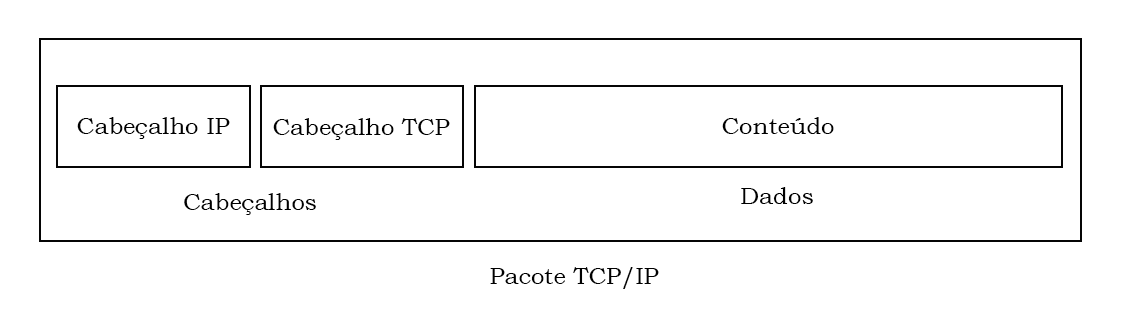
\includegraphics[scale=0.37]{imagens/dados.png}}
\label{fig:exemplo}
\fonte{\citeonline{Jasim}, Adaptado} 
\end{figure}

O conteúdo dentro dos cabeçalhos é essencial para a identificação de ataques, pois possuem informações importantes que podem ser analisadas por IDSs.

\section{Sistema de detecção de intrusão}
Sistema de Detecção de Intrusão (IDS) é um software ou hardware que analisa o trafego de rede buscando comportamentos maliciosos ou violação de regras. Ele funciona analisando os pacotes de rede ou o comportamento dos mesmo para assim identificar anomalias. \cite{CHORAS2021705}

Outra abordagem são os IDSs baseados em Redes Neurais Artificiais (RNA), estes são mais complexos e tem a habilidade de aprender a partir de exemplos, generalização ou dados incompletos \cite{Anitha}. Assim estes podem identificar e aprender quais ações são normais ou maliciosas.

\section{Rede Neural Artificial}
As redes neurais artificiais são técnicas computacionais que usam regras matemáticas incrementais para adquirir conhecimento através de experiencias. Por isso possibilitam trabalhar com modelagem e resolução de
problemas com dados não organizados, treinando, testando e validando um conjunto de dados na entrada visando um objetivo de saída \cite{barros2018avaliaccao},

Para a implementação de um IDS baseado em Redes Neurais Artificiais, é preciso de um modelo de treinamento que ajudará a classificar os pacotes do tráfego de rede. Para isso os dados têm um papel fundamental, quanto mais dados são analisados, melhor será o modelo de treinamento, tornando a base de classificação robusta. % necessita de alterações
 
 % Metodologia
 \chapter{METODOLOGIA}
Para este trabalho, foram utilizados como fonte de dados para o algorítimo, o IDS Kitsune e seus datasets com modelos comums de ataques \cite{kitsune}. A metodologia terá uma abordagem experimental, fazendo o teste em diferentes tipos de ambientes domésticos e hardwares. 

\hfill
\newcolumntype{L}{>{\RaggedRight\arraybackslash}X}
\begin{table}[!hbt]
\renewcommand\thetable{2}
\setlength\tabcolsep{3pt} 
\caption{Hardware utilizado nos testes}
\centering
 \begin{tabularx}{\textwidth}{@{}*{4}{L} @{}} 
 \toprule
 Hardware & RAM & Processamento & Sistema \\ [0.5ex]
 \midrule
 Computador Pessoal &
 16 GB &
 3.6GHz &
 Windows 10 \\ 
 \addlinespace
 Laptop Pessoal &
 8 GB &
 2.30GHz &
 Linux \\ 
 \addlinespace
 Computador Pessoal &
 16GB &
 3.5GHz &
 MacOS \\ 
 \addlinespace
 \bottomrule
\end{tabularx}
\fonte{Autoria Própria, 2022} 
\end{table}

\hfill
\newcolumntype{L}{>{\RaggedRight\arraybackslash}X}
\begin{table}[!hbt]
\renewcommand\thetable{3}
\setlength\tabcolsep{3pt} 
\caption{Dispositivos IoT conectados a Rede}
\centering
 \begin{tabularx}{\textwidth}{@{}*{4}{L} @{}} 
 \toprule
 Dispositivo & Tipo & Fabricante \\ [0.5ex]
 \midrule
 Echo Dot (3ª Geração) &
 Auto falante Inteligente &
 Amazon \\
 \addlinespace
 Camera IP &
 Câmera de Segurança &
 Intelbraz \\
 \addlinespace
 DVR &
 Gravador Digital Inteligente &
 HiLook \\
 \addlinespace
 \bottomrule
\end{tabularx}
\fonte{Autoria Própria, 2022} 
\end{table}

\section{Implantação na Rede Doméstica}
Para a implementação, serão realizados os testes com o IDS instalado diretamente no dispositivo alvo, capturando os pacotes do mesmo, também outra abordagem será a instalação direto no roteador da rede.

\section{ALGORÍTIMO DE DETECÇÃO DE ANOMALIAS}
O algorítimo será implementado em Python3 e adaptado para o uso em ambientes domésticos, utilizando-se de estratégias de análise menos custosas e automatizações, que tornarão o uso menos complexo. 

A implementação do algorítimo e adaptação se dará pela captura automática de pacotes em quantidades baixas (20 mil por análise), para assim tornar o processamento desses pacotes mais rápido. Também, diferentemente do funcionamento do Kitsune, o método de captura, análise e processamento serão de forma automática e recursiva, tornando o processo.

\section{Processamento dos pacotes}
O processamento dos pacotes possui três fases, a primeira captura os pacotes a partir de bibliotecas externas, na segunda fase, o algorítimo gera uma instancia do pacote, com informações como: ip de origem, ip de destino, protocolos, tempo de resposta, etc, e por fim na terceira fase é onde a Rede Neural Artificial Analisa o comportamento de cada instancia.

\section{Exclusão dos arquivos TCPDUMP}
Os arquivos tcpdump gerados, contém informações de pacotes de rede usados durante o processamento dos dados, por isso após seu uso, são excluidos do armazenamento, assim impedindo o acesso não autorizado.

\chapter{CRONOGRAMA}

O desenvolvimento deste trabalho se dará da seguinte forma:

\begin{enumerate}
	\item \label{ela-pro} Elaboração da proposta.
	\item \label{anI} Análise dos métodos de ataques a dispositivos IoT.
	\item \label{anII} Configurações dos ambientes de testes.
	\item \label{anIII} Implementação do algorítimo nos ambientes de teste. 
	\item \label{dI} Análise dos modelos implementados em hardware estudados no item IV.
		\item \label{dII} Validação dos resultados preliminares de desempenho.
	\item \label{tec} Teste e correções.
		\subitem Comparar desempenho entre diferentes ambientes.
	\item \label{esc-tcII} Escrita do TCC II.
\end{enumerate}

\begin{table}[!htbp]
	\centering
		\setlength\tabcolsep{15pt}\begin{tabular*}{\textwidth}{|c @{\extracolsep{\fill}} |c|c|c|c|c|c|c|}
		\hline
		& \multicolumn{5}{c|}{2022}&\multicolumn{2}{c|}{2023} \\
		\hline
		\hspace{-0.4cm} Atvidades \hspace{0.1cm}  & AGO & SET & OUT & NOV & DEZ & JAN & FEV \\
		\hline
		\hspace{-0.3cm}\ref{ela-pro} & X & & & & & & \\
		\hline
		\hspace{-0.3cm}\ref{anI} & & X & X & & & & \\
		\hline	
		\hspace{-0.3cm}\ref{anII} & & & X & & & & \\
		\hline			
		\hspace{-0.3cm}\ref{anIII} & & & X & X & & & \\
		\hline	
		\hspace{-0.3cm}\ref{dI} & & & & & X & & \\
		\hline
		\hspace{-0.3cm}\ref{dII} & & & & & & X & \\
		\hline	
		\hspace{-0.3cm}\ref{tec} & & & & & & & X \\
		\hline	
		\hspace{-0.3cm}\ref{esc-tcII} & & & & & & & X \\
		\hline	
		\end{tabular*}
\end{table} % necessita de alterações
 
 % Resultados
 \chapter{RESULTADOS}
 % necessita de alterações
 
 % Conclusao
 % \chapter{CONCLUSÕES}
A conclusão deve conter os principais aspectos e contribuições de forma a finalizar o trabalho apresentado. Deve-se apresentar o que era esperado do trabalho através dos objetivos inseridos inicialmente e mostrar o que foi conseguido. 

Não se deve inserir um novo assunto na conclusão. Aqui o autor apresentará as próprias impressões sobre o trabalho efetuado. 
    
É importante também que sejam identificadas limitações e problemas que surgiram durante o desenvolvimento do trabalho e quais as consequências do mesmo.

Os trabalhos futuros devem conter oportunidades de expansão do trabalho apresentado, bem como, novos projetos que puderam ser vislumbrados a partir do desenvolvimento do trabalho % necessita de alterações
 
 \postextual
 % Bibliografia
 \bibliography{b_referencias} % necessita de alterações
 
 % Inicia ambiente Apendice
 %\begin{apendicesenv}
 % 
\chapter{Primeiro Apendice}

Teste de apendices

\section{Primeiro Subapendice}
 outro teste de Subapendice
\subsection{Primeiro subapendice}

\subsubsection{Primeiro subsubapendice}
 % necessita de alterações
 %\end{apendicesenv}
 
 % Inicia ambiente Anexo
 %\begin{anexosenv}
 % 

\chapter{Primeiro Anexo}
 % necessita de alterações
 %\end{anexosenv}
 
\end{document}